\chapter{Prototypische Implementierung}
\label{chap:impl}
Dieses Kapitel widmet sich der prototypischen Implementierung der im vorigen Kapitel vorgestellten Konzeption des Frameworks. Als Programmiersprache wird C++ gewählt, da diese Sprache die gesamte Bandbreite der Softwareentwicklung anbietet und sowohl den Zugriff auf die Hardware des Computers als auch die Entwicklung von großen Systemen begünstigt. 

\missing{UMSCHREIBEN}
Die Sprache C++ legt einen Schwerpunkt auf die Sprachmittel zur Entwicklung von Bibliotheken und favorisiert dadurch verallgemeinerte Mechanismen gegenüber in die Sprache integrierten Einzellösungen für typische Problemstellungen.

Eine der Stärken von C++ ist auch die Kombinierbarkeit von effizienter, maschinennaher Programmierung mit mächtigen Sprachmitteln, die einfache bis komplexe Implementierungsdetails zusammenfassen und weitgehend hinter abstrakten Befehlsfolgen verbergen. Dabei kommt vor allem die Template-Metaprogrammierung zum Zuge, eine Technik, die eine nahezu kompromisslose Verbindung von Effizienz und Abstraktion erlaubt.

Als Implementierung des p2p-Netzwerkes wird Chimera \cite{Allen2006Chimera} gewählt, da Pastry selbst als Java-Bibliothek\footnote{\url{http://www.freepastry.org}} verfügbar ist. Die Entwicklung von Tapestry (ebenfalls Java) wurde mit Version 2.01 eingestellt. Chimeras frei verfügbare Code (veröffentlicht unter GPL) und die Kompabilität mit der generischen KBR-API sprechen für Chimera. Somit könnte es bei gravierenden Problemen durch ein anderes Netzwerk ausgetauscht werden, ohne großen Einfluss auf die restlichen Komponenten des System zu haben. Chimera ist der Nachfolger von Tapestry und wird auf der Homepage\footnote{siehe \url{http://current.cs.ucsb.edu/projects/chimera/index.html}} folgendermaßen beschrieben: 
\selectlanguage{english}
\begin{quote}
Chimera is a light-weight C implementation of a \enquote{next-generation} structured overlay that provides similar functionality as prefix-routing protocols Tapestry and Pastry.  Chimera gains simplicity and robustness from its use of Pastry's leafsets, and efficient routing from Tapestry's locality algorithms.  In addition to these properties, Chimera also provides efficient detection of node and network failures, and reroutes messages around them to maintain connectivity and throughput.  
\end{quote}
\selectlanguage{ngerman} 

Das UML-Klassendiagramms in \Fref[plain]{fig:uml} spiegelt den groben Aufbau wieder und zeigt die wichtigsten Klassen. Auf die Darstellung von Hilfskonstrukten wird der Übersichtlichkeit halber verzichtet. Als erster Schritt wird die Anbindung an die Netzwerke erklärt. Danach wird -- ausgehend von der Applikation -- die Implementierung des Publish/Subscribe-Systems erläutert. Angewandte Techniken wie \ac{tmp} oder \emph{policy based}-Design werden im Anhang dieser Arbeit beschrieben. Sie werden benötigt um den zusätzlichen Verwaltungsaufwand zur Laufzeit durch geschickte Anwendung des zur Übersetzungszeit vorhandenen Wissens zu minimieren. Das nutzbare Wissen umfasst beispielsweise die Typen der Events oder die zur Optimierung ausgewählten Strategien und deren Besonderheiten.

\texttt{P2PInterface} ist eine abstrakte Basisklasse und repräsentiert die in \cite{Dabek2003Towards} beschriebene \ac{kbr}-API. Aktuell wird diese durch die Klasse \texttt{ChimeraWrapper} implementiert, welche über die Klasse \texttt{ChimeraWrapperImpl} Zugriff auf das Netzwerk Chimera bietet. Hier wurde das \enquote{PIMPL}-Pattern angewandt, mit dem die eigentliche Implementierung versteckt werden kann \cite{Alexandrescu2001Modern}. Damit werden die Implementierungsdetails, wie interne Datentypen oder Methoden, vor dem Nutzer versteckt und müssen demnach nicht im zu inkludierenden Header angegeben werden. Diese können nun nach belieben geändert werden ohne dass der Nutzer neukompilieren muss, da sich die Schnittstelle nicht verändert. Als Nebeneffekt sinkt die Übersetzungzeit, da insgesamt weniger Header inkludiert und geparst werden müssen.

Zur Vereinfachung werden sämtliche Identifikationsdaten, zum Beispiel die Adresse eines Knotens, des Netzwerkes als \texttt{std::string} repräsentiert. Dies entbindet den Entwickler der Implementierung weiterer Wrapperklassen von komplexen Hilfskonstrukten. Zur eigentlichen Nachrichtenübertragung wird der Datentyp \texttt{std::vector$<$char$>$}, die objektorientierte Version eines \texttt{char*}, bereitgestellt. Neben der einfacheren Zugriffsweise, bietet dies zusätzlichen Schutz gegen einen pufferüberlauf und ähnliche Probleme.\\
Weitere Netzwerke können auf einfache Art und Weise durch entsprechende Wrapperklassen eingebunden werden.

\begin{figure}[htbp]
\centering
\resizebox{\textwidth}{!}{%
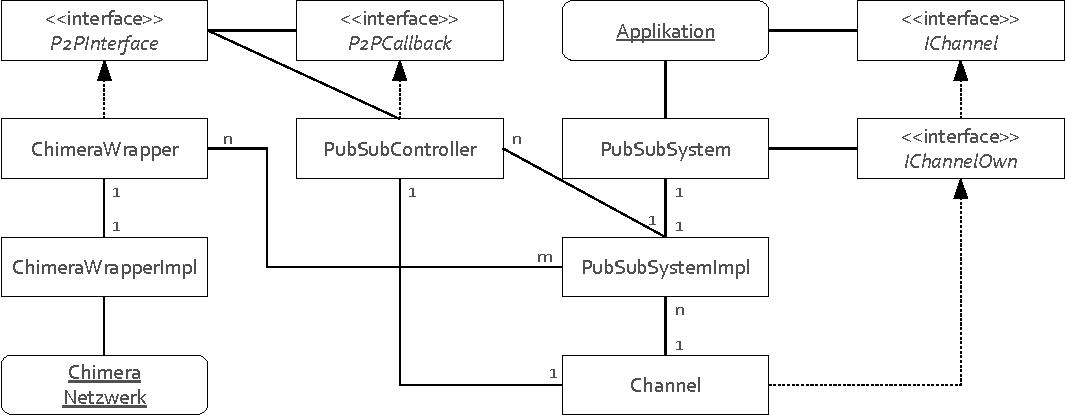
\includegraphics{grafics/uml.pdf}}
\caption{Vereinfachtes Klassendiagramm des Frameworks}
\label{fig:uml}
\end{figure}

Die \texttt{Applikation} greift auf das Publish/Subscribe-System über den Singleton \texttt{PubSub\-Sytem} zu. Beiden ist der optimierte \texttt{Channel} nur über die abstrakten Basisklassen \texttt{IChannel} beziehungsweise \texttt{IChannelOwn} zugänglich. Diese sind in \Fref[plain]{lst:interface_channel} dargestellt und bieten lediglich die drei üblichen Methoden\footnote{\texttt{subscribe}, \texttt{unsubscribe} und \texttt{publish}} für Publish/Subscribe-Systeme an und verdecken dadurch die Komplexität der Klasse \texttt{Channel} vor dem Benutzer. Bei der Anmeldung an einem Kanal muss ein Funktionspointer vom Typ \texttt{app\_deliver\_func} übergeben werden. Diesem übergibt das Publish/Subscribe-System eine empfangene Nachricht und liefert damit die Events an die Applikation aus. Der Anmeldung kann ebenfalls ein Prädikat zur Filterung übergeben werden falls die gewählten Strategien dies unterstützen. \texttt{Channel} selbst ist eine mit policy-based Design erstellte Templateklasse\footnote{siehe \Fref{chap:impl_tmp} im Anhang zur Erklärung} und bekommt die verschiedenen Strategien -- in \Fref{fig:uml} ebenfalls nicht dargestellt -- als Policies übergeben. \ac{tmp} ermöglicht es zudem jede \texttt{Channel}-Instanz auf die gewählten Policies abzustimmen. Weiterhin wird für jeden \texttt{Channel} ein optimierter Header erzeugt, dessen Größe an Nutzlast für Verwaltungsdaten von den gewählten Policies abhängig ist. Durch diese Maßnahmen wird der Overhead zur Laufzeit stark reduziert. 

\lstinputlisting[caption={Schnittstellen für die Klasse \texttt{Channel}}, label=lst:interface_channel, float=!t]{listings/interface_channel.h}

Die Klasse \texttt{PubSubController} implementiert das Interface \texttt{P2PCallback} und kann sich somit für die Callbacks des Netzwerkes registrieren. Der PubSubController ist die Schnittstelle des Publish/Subscribe-Systems mit dem \ac{p2p}-Netzwerk und bietet die benötigte Funktionalität für die Klasse Channel. Zudem werden die ankommenden Nachrichten in deliver über eine Queue und einen Dispatch-Thread an die einzelnen Kanäle verteilt. 

\texttt{PubSubSystemImpl} kennt die verschiedenen Netzwerkwrapper (in \Fref{fig:uml} ist dies \texttt{ChimeraWrapper}) und besitzt für jeden optimierten \texttt{Channel} eine Klassenvariable als \texttt{IChannelOwn*}. Auf diese hat die Klasse \texttt{PubSubSystem} als \texttt{friend class}\footnote{\enquote{friend} ist eine besondere Beziehung zwischen zwei Klassen} freien Zugriff und kann die Methodenaufrufe an der Publish/Subscribe-API an die einzelnen Instanzen der Klasse \texttt{Channel} weiterleiten. Für jedes genutzte Netzwerk instantiiert \texttt{PubSubSystemImpl} einen eigenen \texttt{PubSubController} und übergibt diesen an die entsprechenden Kanäle. Mit verschiedenen Instanzen der Klasse \texttt{PubSubController} können somit auch verschiedene Netzwerke angesprochen und entsprechend der Optimierungsmetriken für verschiedene Kanäle genutzt werden.

Im Optimierungsschritt müssen folgende Klassen generiert oder teilweise angepasst werden:
\begin{description}
\item[ChannelList.h] In dieser Datei ist eine Liste der vorhandenen Kanäle in einem \texttt{enum} abgelegt. Die Einträge dienen der Auswahl des Kanals bei der Kommunikation mit dem \texttt{PubSubSytem}. Durch das enum wird ein einfach zu überprüfendes Mapping auf den eigentlichen Kanal ermöglicht.
\item[PubSubSystemImpl.h] Diese Klasse muss komplett generiert werden. Sie hat Zugriff auf alle zur Optimierung genutzten Strategien und den daraus erzeugten Instanzen der Templateklasse \texttt{Channel}. Zudem können hier die verschiedenen Netzwerke mit den verschiedenen Kanälen über Instanzen der Klasse \texttt{PubSubController} verbunden werden.
\item[PubSubSystem.cpp] Die Klasse \texttt{PubSubSystemImpl} und damit auch die optimierten Kanäle werden erst im Optimierungsschritt erzeugt. Daher müssen die Zugriffsmethoden auf die im \texttt{PubSubSystemImpl} enthaltenen Kanäle ebenfalls im Optimerungsschritt generiert werden.
\end{description}

Dank der strikten Aufteilung der Klassen beim Netzwerk und dem Publish/Subscribe-System wird die Nutzerfreundlichkeit des Frameworks aus Entwicklersicht ermöglicht, wie es das Codebeispiel im nächsten Abschnitt darlegt. Hier ist deutlich zu sehen, dass der Nutzer keinerlei Wissen über das genutzte Netzwerk noch über die zur Optimierung herangezogenen Strategien haben muss, um das System benutzen zu können.

\section*{Zugriff auf M$^2$etis aus Benutzersicht}
Das \Fref[plain]{lst:pubsub_usage} zeigt den Zugriff der Applikation auf das Publish/Subscribe-System. Der Code erzeugt drei Knoten, die mit dem System arbeiten. Der erste Knoten sendet Nachrichten auf dem Kanal \texttt{ANY\_ALL}\footnote{Der Name \enquote{ANY\_ALL} suggeriert, dass hier jegliche Art von Nachrichten an alle Knoten verteilt werden.}, für den sich die beiden anderen Knoten anmelden. In den Zeilen 10 bis 12 ist die Empfangsfunktion definiert, welche dem System bei Anmeldungen übergeben werden muss. Diese Funktion wird in den Zeilen 18 und 21 mittels \texttt{boost::bind} an die benötigte Signatur angepasst und mit Metadaten (hier der Knotenname) angereichert. Das System wird in den Zeilen 15 und 16 initialisiert und ein Handle auf den Kanal \texttt{ANY\_ALL} erlangt. Die Anmeldung der Knoten erfolgt in den Zeilen 19 und 22, mit Angabe eines im Netzwerk bekannten Knoten zum Einstieg in das Netzwerk und der Empfangsfunktion. In den Zeilen 24\,-\,27 wird in einer Endlosschleife eine Nachricht über das Handle in das System gebracht und fünf Sekunden geschlafen.


\lstinputlisting[caption={Zugriff auf M$^2$etis aus Benutzersicht}, label=lst:pubsub_usage, float=!t]{listings/pubsub_usage.cpp}

Dieses Codebeispiel zeigt deutlich die Kapselung des komplexen optimierten Publish/\-Subscribe-Systems und dessen einfache und unkomplizierte Handhabbarkeit. Über \texttt{boost::bind} können beliebige Methoden an die Signatur der Empfangsfunktion angepasst werden. Daher muss die Applikation einerseits nicht von einer abstrakten Basisklasse abgeleitet sein und andererseits bleibt die eigentliche Empfangsfunktion anpassbar, wie es im Codebeispiel dargestellt ist.

